%!TEX root = abschlusspraesentation.tex

\begin{frame}[c]\frametitle{NN Auswertung}
\usetikzlibrary{arrows}
\usetikzlibrary{positioning} 
\usetikzlibrary{automata} 

  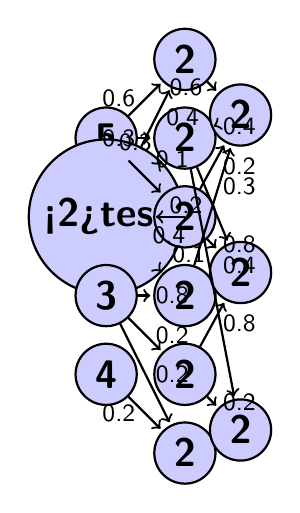
\begin{tikzpicture}[->,shorten >=1pt,auto, node distance=1cm,
    thick,main node/.style={circle,fill=blue!20,draw,font=\sffamily\Large\bfseries}]

    \node[main node] (0) {5};
    \node[main node] (1) [below of=0] {\only<2>{test}};
    \node[main node] (2) [below of=1] {3};
    \node[main node] (3) [below of=2] {4};

    \node[main node] (11) [right of=0] {2};
    \node[main node] (10) [above of=11] {2};
    \node[main node] (12) [right of=1] {2};
    \node[main node] (13) [right of=2] {2};
    \node[main node] (14) [right of=3] {2};
    \node[main node] (15) [below of=14] {2};

    \node[main node] (20) [below right  of=10] {2};
    \node[main node] (21) [below right  of=12] {2};
    \node[main node] (22) [below right  of=14] {2};

    \path[every node/.style={font=\sffamily\small}]
      (0) edge node [left] {0.6} (10)
          edge node[left] {0.3} (11)
          edge node {0.1} (12)
      (1) edge node [right] {0.4} (10)
          edge node {0.3} (11)
          edge node {0.4} (12)
          edge node {0.1} (13)
      (2) edge node [right] {0.8} (13)
          edge node [right] {0.2} (14)
          edge node [right] {0.2} (15)
      (3) edge node [left] {0.2} (15)

      (10)edge node [left] {0.6} (20)
      (11)edge node [right] {0.4} (20)
          edge node {0.3} (21)
          edge node {0.4} (22)
      (12)edge node [right] {0.8} (21)
          edge node [right] {0.2} (20)
      (13)edge node [left] {0.2} (20)
      (14)edge node [right] {0.8} (21)
          edge node [right] {0.2} (22)
      ;
  \end{tikzpicture}    
\end{frame}
